\documentclass[10pt,pdf,hyperref={unicode}, dvipsnames]{beamer}
%!TEX root = ../presentation.tex
\usepackage[english,russian]{babel}
% \usepackage[T2A,T1]{fontenc}
\usepackage[utf8]{inputenc}
% \usepackage{tikz}
\usepackage[unicode]{hyperref}
% \usepackage{pgfplots,standalone}
\usepackage{caption}
\usepackage[normalem]{ulem}
\usepackage
	{
		% Дополнения Американского математического общества (AMS)
		amssymb,
		amsfonts,
		amsmath,
		amsthm,
		physics
		}
% \usepackage{lmodern}
% \pgfplotsset{compat=newest} 
% \usetikzlibrary{%
%     decorations.pathreplacing,%
%     decorations.pathmorphing,%
%     patterns,%
%     angles,%
%     quotes,%
%     calc, %
%     3d, %
%     backgrounds, %
%     positioning%
% }


% Стиль презентации

 \usetheme{default}
 \usefonttheme{professionalfonts}
 \usecolortheme{}
 % \usecolortheme{whale}
% \let\oldframe\enumerate
% \renewcommand{\frame}{%
% \oldframe
% \let\olditemize\itemize
% \renewcommand\itemize{\olditemize\addtolength{\itemsep}{100pt}}%
% }
 

% \setbeamercolor{frametitle right}{fg=white,bg=Brown!85}
% \setbeamercolor{frametitle}{fg=white,bg=Brown!85}
%\setbeamercolor{frametitle right}{fg=white,bg=black!85} %
\setbeamercolor{frametitle}{fg=white,bg=black!85} % Цвет титульника
\setbeamercolor{item projected}{fg=white,bg=black!85} % Цвет титульника
\setbeamertemplate{blocks}[rounded][shadow=false] %стиль блоков
\setbeamertemplate{itemize item}{\color{black!85}$\bullet$}
\setbeamertemplate{headline}{}
\setbeamertemplate{footline}{} 
\setbeamertemplate{navigation symbols}{} % минус навигация
% \let\Tiny=\tiny % решает проблему со шрифтами в TexLive
%\setbeamertemplate
%	{footline}{
%		\color{black!40!white}
%		\quad\hfill
%		\insertframenumber/\inserttotalframenumber
%		\hfill\vspace{1cm}\quad
%	} 


\beamersetrightmargin{1cm} 
\beamersetleftmargin{1cm}

\setbeamertemplate{enumerate item}
{
	\usebeamercolor[bg]{item projected}
	\raisebox{1pt}{\colorbox{black!85}{\color{fg}\footnotesize\insertenumlabel}}%
}

% \setbeamertemplate{itemize item}{%
% 	\usebeamercolor[bg]{item projected}%
% 	\raisebox{3pt}{{\colorbox{black!85}\footnotesize$\bf$\bullet}}%
% }

\setbeamercolor{item projected}{bg=black,fg=white}
\setbeamercolor{title}{bg=black!85,fg=white}

\setbeamertemplate{frametitle}
{	
	\nointerlineskip
	\begin{beamercolorbox}[sep=15pt,ht=1.9em,wd=\paperwidth]{frametitle}
		% \vspace{}%
		\strut\insertframetitle\strut
		\vskip-1.8ex%	
	\end{beamercolorbox}
}


\usepackage{mathtools}
\mathtoolsset{showonlyrefs=true} 

\usepackage{import}
\usepackage{pdfpages}
\usepackage{transparent}
\usepackage{xcolor}
\usepackage{calc}

\newcommand{\executeiffilenewer}[3]{%
    \ifnum\pdfstrcmp{\pdffilemoddate{#1}}%
    {\pdffilemoddate{#2}}>0%
    {\immediate\write18{#3}}\fi%
}
\newcommand{\includesvg}[1]{%
    \executeiffilenewer{#1.svg}{#1.pdf}%
    {inkscape -z -D --file=#1.svg %
    --export-pdf=#1.pdf --export-latex}%
    \import{./fig/}{#1.pdf_tex}
}

\usepackage{caption}
\usepackage{subcaption}
\renewcommand{\phi}{\varphi}
%\usepackage[e]{esvect}
%\usepackage{animate}
%\renewcommand{\vec}{\vv}
\newcommand{\tM}{\widetilde{M}}
\begin{document}
\title[Моделирование морской поверхности]{Численное моделирование морской поверхности}

\author{Понур К.А.}

\institute{Национальный исследовательский Нижегородский государственный университет имени Н. И. Лобачевского \\ Радиофизический факультет}

%!TEX root = ..\presentation.tex
\begin{frame}[plain]
	\begin{center}
		\small{\insertinstitute}
		\vspace{1cm}
	\end{center}
		\begin{beamercolorbox}[sep=8pt,center]{title}
			\usebeamerfont{title}\inserttitle
		\end{beamercolorbox}
		\vspace{0.1cm}
	\begin{flushright}
		\normalsize \textbf{Работу выполнил:}\\
		\large
		\insertauthor \\
		\vspace{0.5cm}
		\normalsize{\textbf{Научный руководитель:}\\}
		\large{Караев В.Ю.}
		\vfill
	\end{flushright}

	\centering{\small{\today }}
\end{frame}


% \section{Введение}
% \subsection{Цели работы}
\begin{frame}[t]
	\frametitle{Введение}
	\vfill
	\textbf{Цели: }\\
		% \vfill
		\begin{enumerate}
			% \item \sout{Получить зачёт по УНЭ.}
			\item Изучить принципы моделирования морской поверхности.

			\item Оптимизировать существующие алгоритмы.


		\end{enumerate}
		\vfill
% \end{frame}
% \subsection{Актуальность работы}
% \begin{frame}[t]

	\textbf{Актуальность работы: }

	\begin{enumerate}
		% \item Проведение испытаний оборудования до его изготовления
		\item Тестирование и разработка алгоритмов восстановления океанографической информации
		\item Оценка возможностей новых радиолокаторов
		\item Постановка численных экспериментов, в частности накопление статистических данных
	\end{enumerate}
	\vfill
\end{frame}

% \begin{frame}[t]\frametitle{Основные понятия}

% Для статистически однородного и стационарного поля $\zeta$ высот морского волнения справедливо следующее выражение для его корреляционной функции:

% \begin{equation}
%  M(\rho) = \langle{\zeta(r)\zeta(r+\rho)}\rangle.
% \end{equation}

% Она связана с спектром высот $S(k)$ морской поверхности:
% \begin{equation}
%     	M(\rho)=\int\limits_0^{\infty} S(k)\cos(k \rho) \dd{k},
% \end{equation}    
% Спектр уклонов морской поверхности связан со спектром высот соотношением $S_{\theta}(k)=k^2 S(k)$.

% Корреляционная функция наклонов:
% \begin{equation}
% 	M_{\theta}(\rho)=\int\limits_0^{\infty} k^2 S(k)\cos(k \rho) \dd{k}
% \end{equation}
%     % Если поверхность представляем как $\zeta(r)= \sum\limits_{i=1}^N a_i\cos(k_i r+ \phi)$, то корреляционная функция модельного поля определяется выражением: 
%     % \begin{equation}
%     % 	\tM(\rho)=\sum\limits_0^{N} b_i \cos(k_i \rho), \quad b_i=\frac{a_i^2}{2},
%     % \end{equation}
%     % $k_i$ -- абсцисса спектральной компоненты
 
%     % $b_i$ -- ордината спектральной компоненты

% \end{frame}

\begin{frame}[t]\frametitle{Одномерное моделирование}
\vskip -10pt
Одномерную поверхность представим как:
\begin{equation}
	\zeta(r, t)= \sum\limits_{i=1}^N a_i\cdot 
		\cos(k_ir + \psi_{i}),
\end{equation}
где $\psi_i$ -- случайная фаза, $a_i$ -- амплитуда $i$-ой гармоники

Корреляционная функция такого поля запишется как: 
    \begin{equation*}
    	\tM(\rho)=\sum\limits_0^{N} b_i \cos(k_i \rho)
    \end{equation*}


\vskip -12pt
\begin{figure}[H]
	\begin{minipage}{0.49\linewidth}
			\centering
			%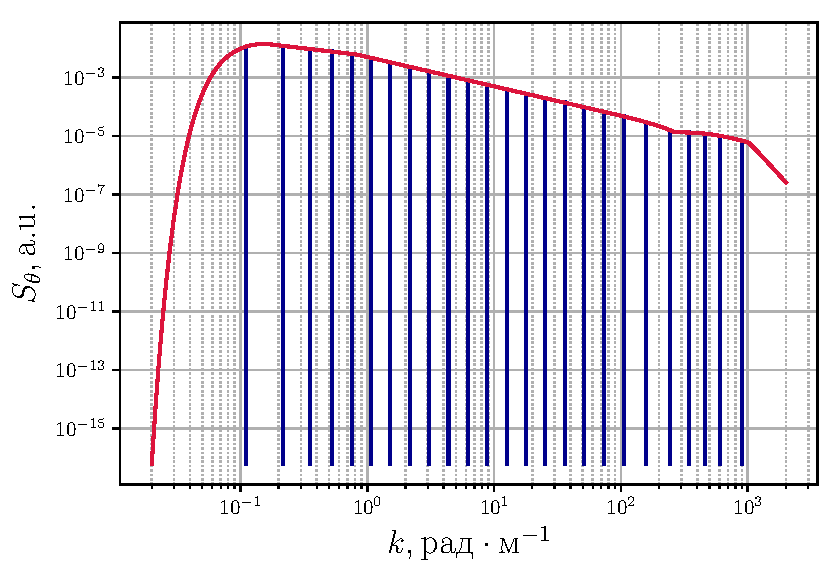
\includegraphics[width=\linewidth]{fig/split_angles}
			\caption{Пример расположения спектральных компонент}	
	\end{minipage}
	\hfill
	\begin{minipage}{0.49\linewidth}
		АКФ реального поля:
		\begin{equation}
			M(\rho)=\int\limits_0^{\infty} S(k)\cos(k \rho) \dd{k},
		\end{equation}
		$S(k)$ -- спектр морской поверхности \\
	    $k_i$ -- абсцисса спектральной компоненты
 
    	
	\end{minipage}
	\label{fig:splits}		
\end{figure}

\end{frame}
\begin{frame}[t]\frametitle{Эквидистантное расположение}
	\begin{figure}[h!]
		\begin{minipage}{0.49\textheight}
				\centering
				%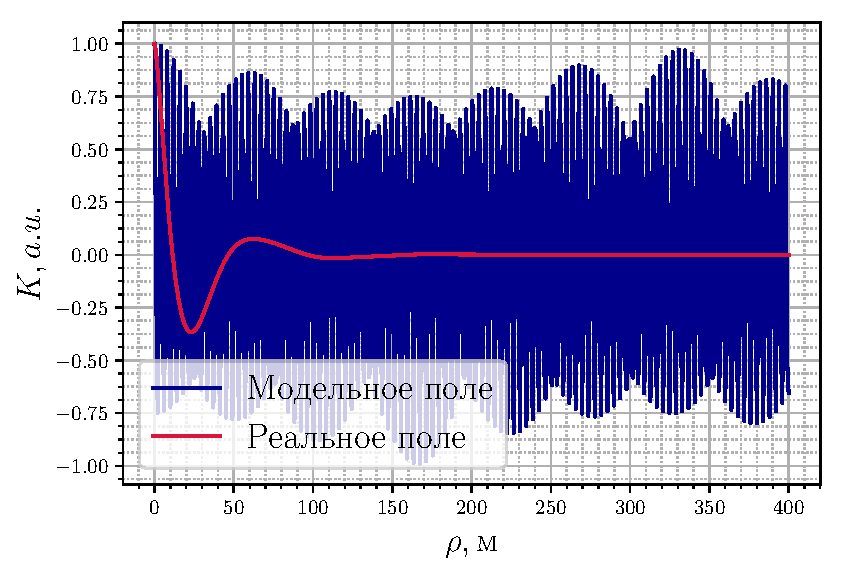
\includegraphics[width=\linewidth]{fig/correlation_height_lin.pdf}
				\label{fig:ch0}		
		\end{minipage}
		\hfill
		\begin{minipage}{0.49\linewidth}
				\centering
				%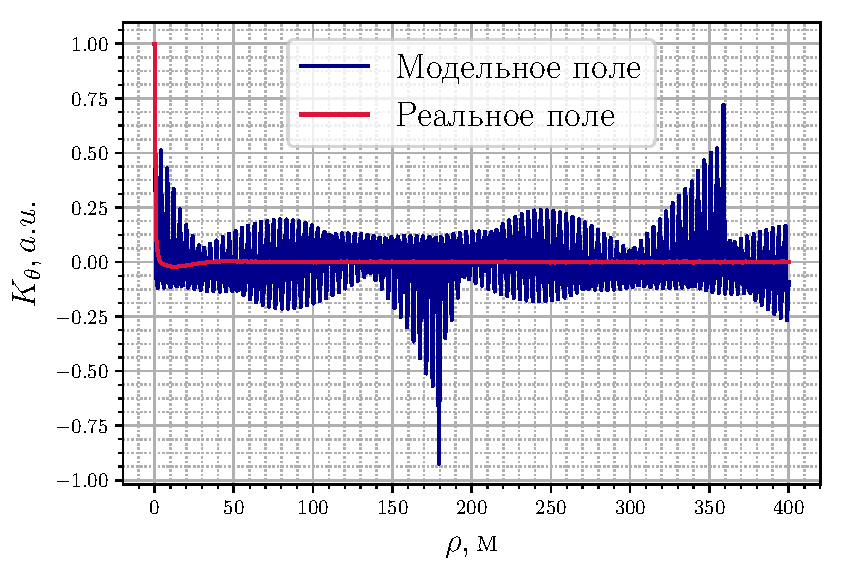
\includegraphics[width=\linewidth]{fig/correlation_angles_lin.pdf}
		\end{minipage}
		\caption{Корреляционные функции высот и уклонов при эквидистантном расположении узлов. $U=10 \frac{\text{м}}{\text{c}}$, $N=256$}
				\label{fig:ca0}		
	\vspace{-20pt}
	\end{figure}
	Узлы задаются выражением
	\begin{equation}
		k_i=\Delta k\cdot i
	\end{equation}
	\begin{equation*}
	b_i = \int\limits_{(i-1)\Delta k}^{i \Delta k} S(k) \dd{k} -
	\text{амплитуда спектральной компоненты}
	\end{equation*}

% \begin{equation}
% 	M(0)=\sigma^2=\int\limits_0^{\infty} S(k) \dd{k}
% \end{equation}

\end{frame}


\begin{frame}[t]\frametitle{Эквидистантное расположение}
	При очень большом числе гармоник период функций корреляции всё ещё недостаточно большой
	\begin{figure}[h!]
		\vfill
		\begin{minipage}{0.49\textheight}
				\centering
				%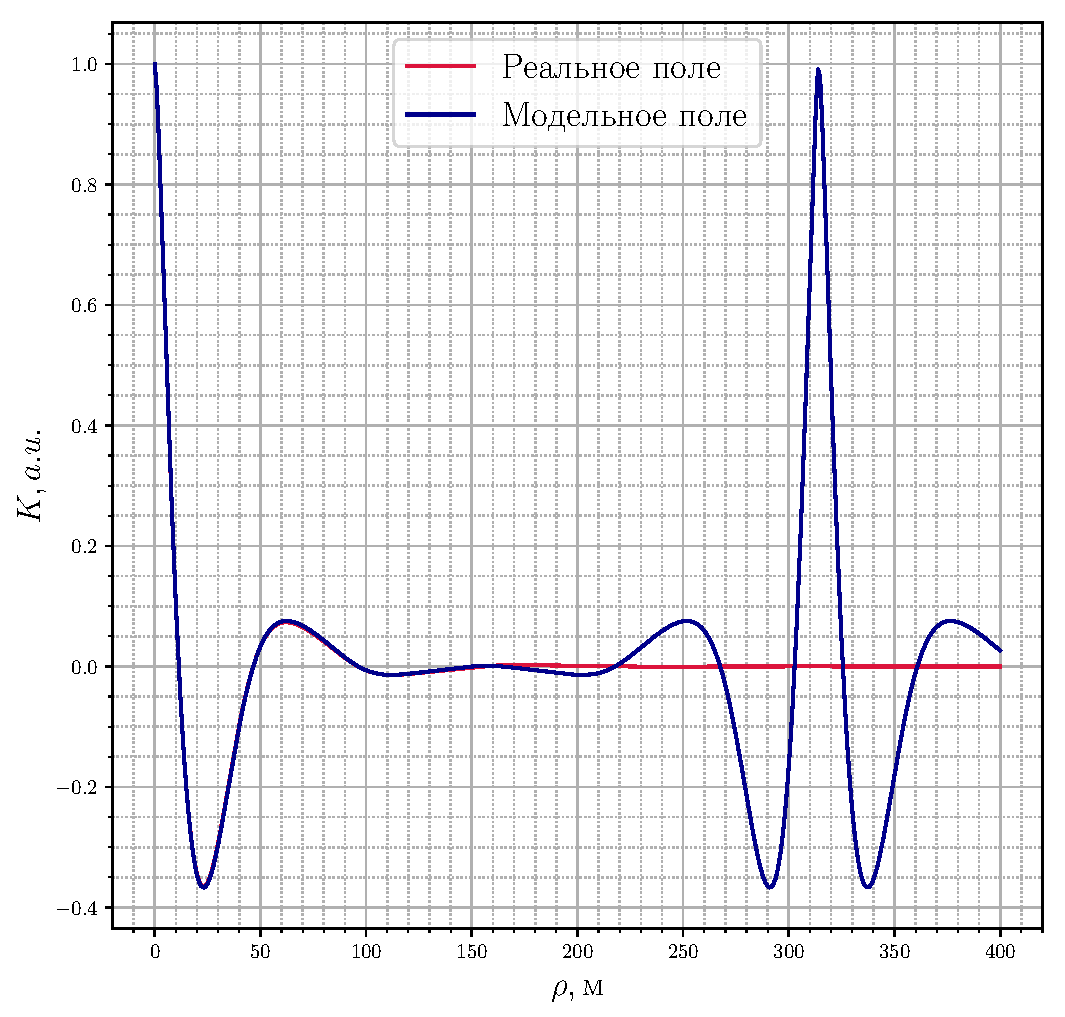
\includegraphics[width=\linewidth]{fig/correlation_height5_slopes2.pdf}
		\end{minipage}
		\hfill
		\begin{minipage}{0.49\linewidth}
				\centering
				%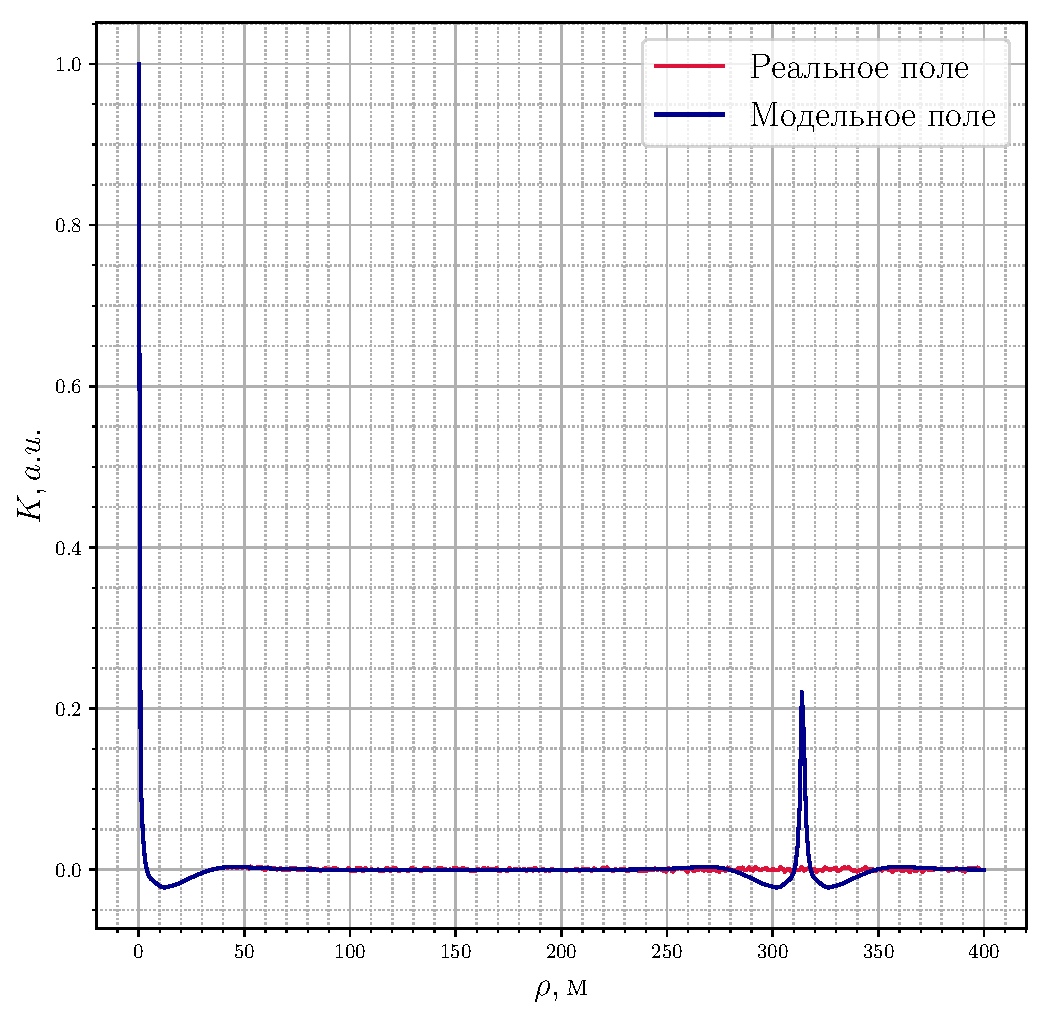
\includegraphics[scale=0.26]{fig/correlation_angles5_slopes2.pdf}
		\end{minipage}
		\caption{Корреляционные функции высот и уклонов при эквидистантном расположении узлов. $U=10 \frac{\text{м}}{\text{c}}$, $N=10^5$}
		\label{fig:ca05}		


	\end{figure}


% \begin{equation}
% 	M(0)=\sigma^2=\int\limits_0^{\infty} S(k) \dd{k}
% \end{equation}

\end{frame}


\begin{frame}[t]\frametitle{Неэквидистантное расположение}
    
\begin{figure}[h!]
	\begin{minipage}{0.49\linewidth}
			\centering
			%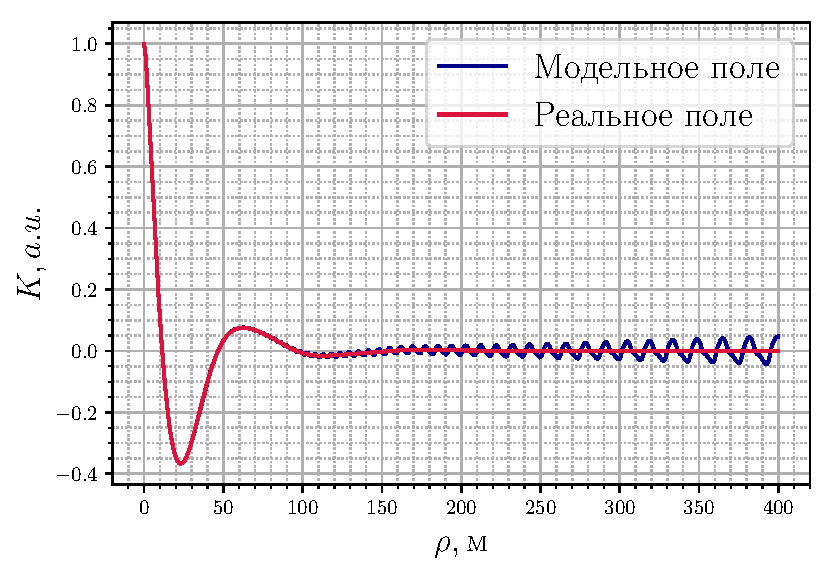
\includegraphics[width=\linewidth]{fig/correlation_height_log.pdf}
			\label{fig:ch1}		
	\end{minipage}
	\hfill
	\begin{minipage}{0.49\linewidth}
			\centering
			%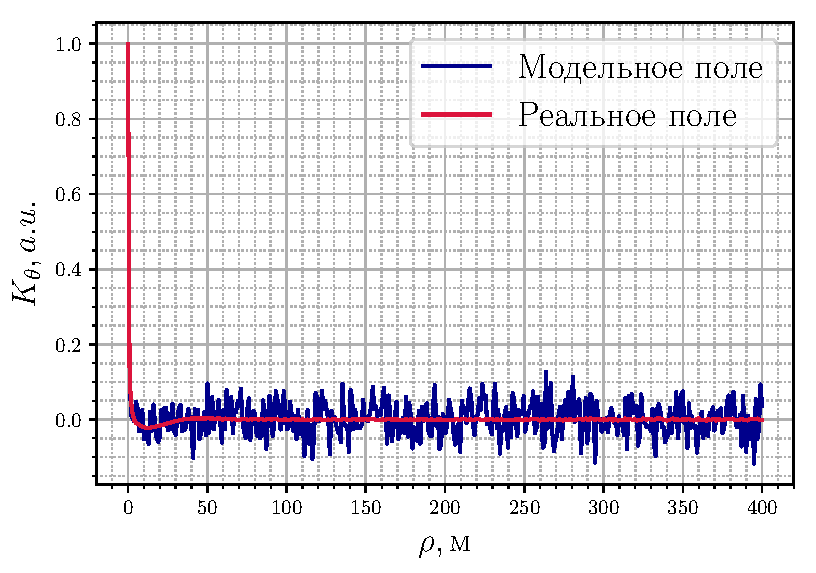
\includegraphics[width=\linewidth]{fig/correlation_angles_log.pdf}
			\label{fig:ca1}		
	\end{minipage}
	\caption{Корреляционные функции высот и уклонов при логарифмическом расположении узлов. $U=10 \frac{\text{м}}{\text{c}}$, $N=256$}
\end{figure}
	Узлы задаются выражением
	\begin{equation}
		k_i=10^{i \Delta k}
	\end{equation}
	\begin{equation*}
	b_i = \int\limits_{10^{(i-1)\Delta k}}^{10^{i \Delta k}} S(k) \dd{k} -
	\text{амплитуда спектральных компонент}
	\end{equation*}

\end{frame}



\begin{frame}[t]
\frametitle{<<Отбеливание>> спектра}
    Предположим, что гармонические составляющие при больших $\rho$ складываются <<некогерентным>> образом. То есть  мощность шума определяется как
    \begin{equation}
    	\sigma^2_{noise}= \sum_{i=1}^N \frac{b_i^2}{2}
    \end{equation}
    В области малых $\rho$ гармоники суммируются <<когерентно>> и соответствующая мощность равна
    \begin{equation}
    	\tM^2(0)=\qty(\sum_{i=1}^N b_i)^2
    \end{equation}
    Введем функцию, характеризующую относительную мощность шумов
    \begin{equation}
    	\label{eq:Q}
    	Q=\frac{\sigma^2_{noise}}{\tM^2(0)}
    \end{equation}


\end{frame}
\begin{frame}[t]
    \frametitle{<<Отбеливание>> спектра}
	Минимизируем величину \eqref{eq:Q}, решая систему уравнений
    \begin{equation}
    	\begin{cases}
    		\pdv{Q}{b_1}=0 \\
    		\hfill \vdots \hfill\\
    		\pdv{Q}{b_N}=0, \\
    	\end{cases} \qquad \text{ где } \pdv{Q}{b_i}=\frac{b_i}{\qty (\sum\limits_{i=1}^{N} b_i)^2} - \frac{\sum\limits_{i=1}^{N} b_i^2}{\qty (\sum\limits_{i=1}^{N} b_i)^3}
    \end{equation}
    Она сводится к следующей системе  $b_i \sum\limits_{i=1}^{N} b_i -\sum\limits_{i=1}^{N} b_i^2=0 $
    \vfill
    Частным результатом решения является $b_1=b_2=\dots=b_N$.
    \vfill
    % Задача сводится к разбиению области определения спектра на участки $\Delta k_i$, интегралы по которым от функции $S(k)$ имеют одинаковые значения.

    \begin{equation}
   \text{Для высот:}\quad 	b_i=b_1= \frac{M(0)}{N}=\frac1N \int\limits_0^{\infty} S(k) \dd{k}
    \end{equation}

    \begin{equation}
    \text{Для наклонов:}\quad 	b^{\theta}_i=b^{\theta}_1= \frac{M^{\theta}(0)}{N}=\frac1N \int\limits_0^{\infty} k^2S(k) \dd{k}
    \end{equation}

\end{frame}



\begin{frame}[t]
    \frametitle{<<Отбеливание>> спектра}
    Потребуем сопряжения в нуле всех производных  функций
    $\tM(\rho)$ и $M(\rho)$. 
    Для функции корреляции стационарной случайной функции $M(\rho)$ справедливо
    \begin{equation}
    	M'_{\rho}=\pdv[2]{M(\rho)}{\rho}=\int\limits_{0}^{\infty} k^2 S(k)\cos(k \rho)\dd{k}
    \end{equation}
    А значит можно переписать наше требование в виде
 \begin{equation}
	\sum_{i=1}^N b_ik_i^{2p}=\int\limits_{0}^{\infty} k^{2p}S(k)\dd{k}, p = 1,2,\dots,N.
\end{equation}
Решать такую систему довольно сложно, поэтому потребуем выполнение более простого равенства
\begin{equation}
	\sum_{i=1}^N b_ik_i^{2}=\int\limits_{0}^{\infty} k^{2}S(k)\dd{k}
\end{equation}


\end{frame}


\begin{frame}[t]\frametitle{Детерминированное расположение узлов}
    

\begin{minipage}{0.49\linewidth}
\centering Для наклонов:
\begin{equation*}
	k_i=\sqrt\frac{N}{{\int\limits_{0}^{\infty} k^2 S(k) \dd{k}}}\cdot {\int\limits_{\Delta k_i} k^4 S(k) \dd{k}}
	\label{eq:ki}
\end{equation*}
\end{minipage}
\hfill
\begin{minipage}{0.49\linewidth}
\centering Для высот:
	\begin{equation*}
	k_i=\sqrt\frac{N}{{\int\limits_{0}^{\infty} S(k) \dd{k}}}\cdot \int\limits_{\Delta k_i} k^2 S(k) \dd{k}
	\label{eq:ki}
\end{equation*}
\end{minipage}
\vfill
\begin{figure}[H]
	\begin{minipage}{0.49\linewidth}
			\centering
			%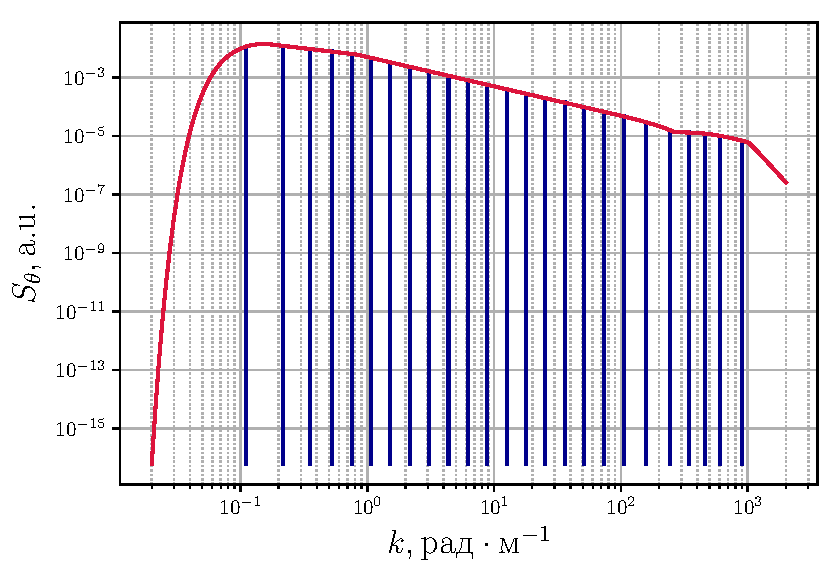
\includegraphics[width=\linewidth]{fig/split_angles}	
	\end{minipage}
	\hfill
	\begin{minipage}{0.49\linewidth}
			\centering
			%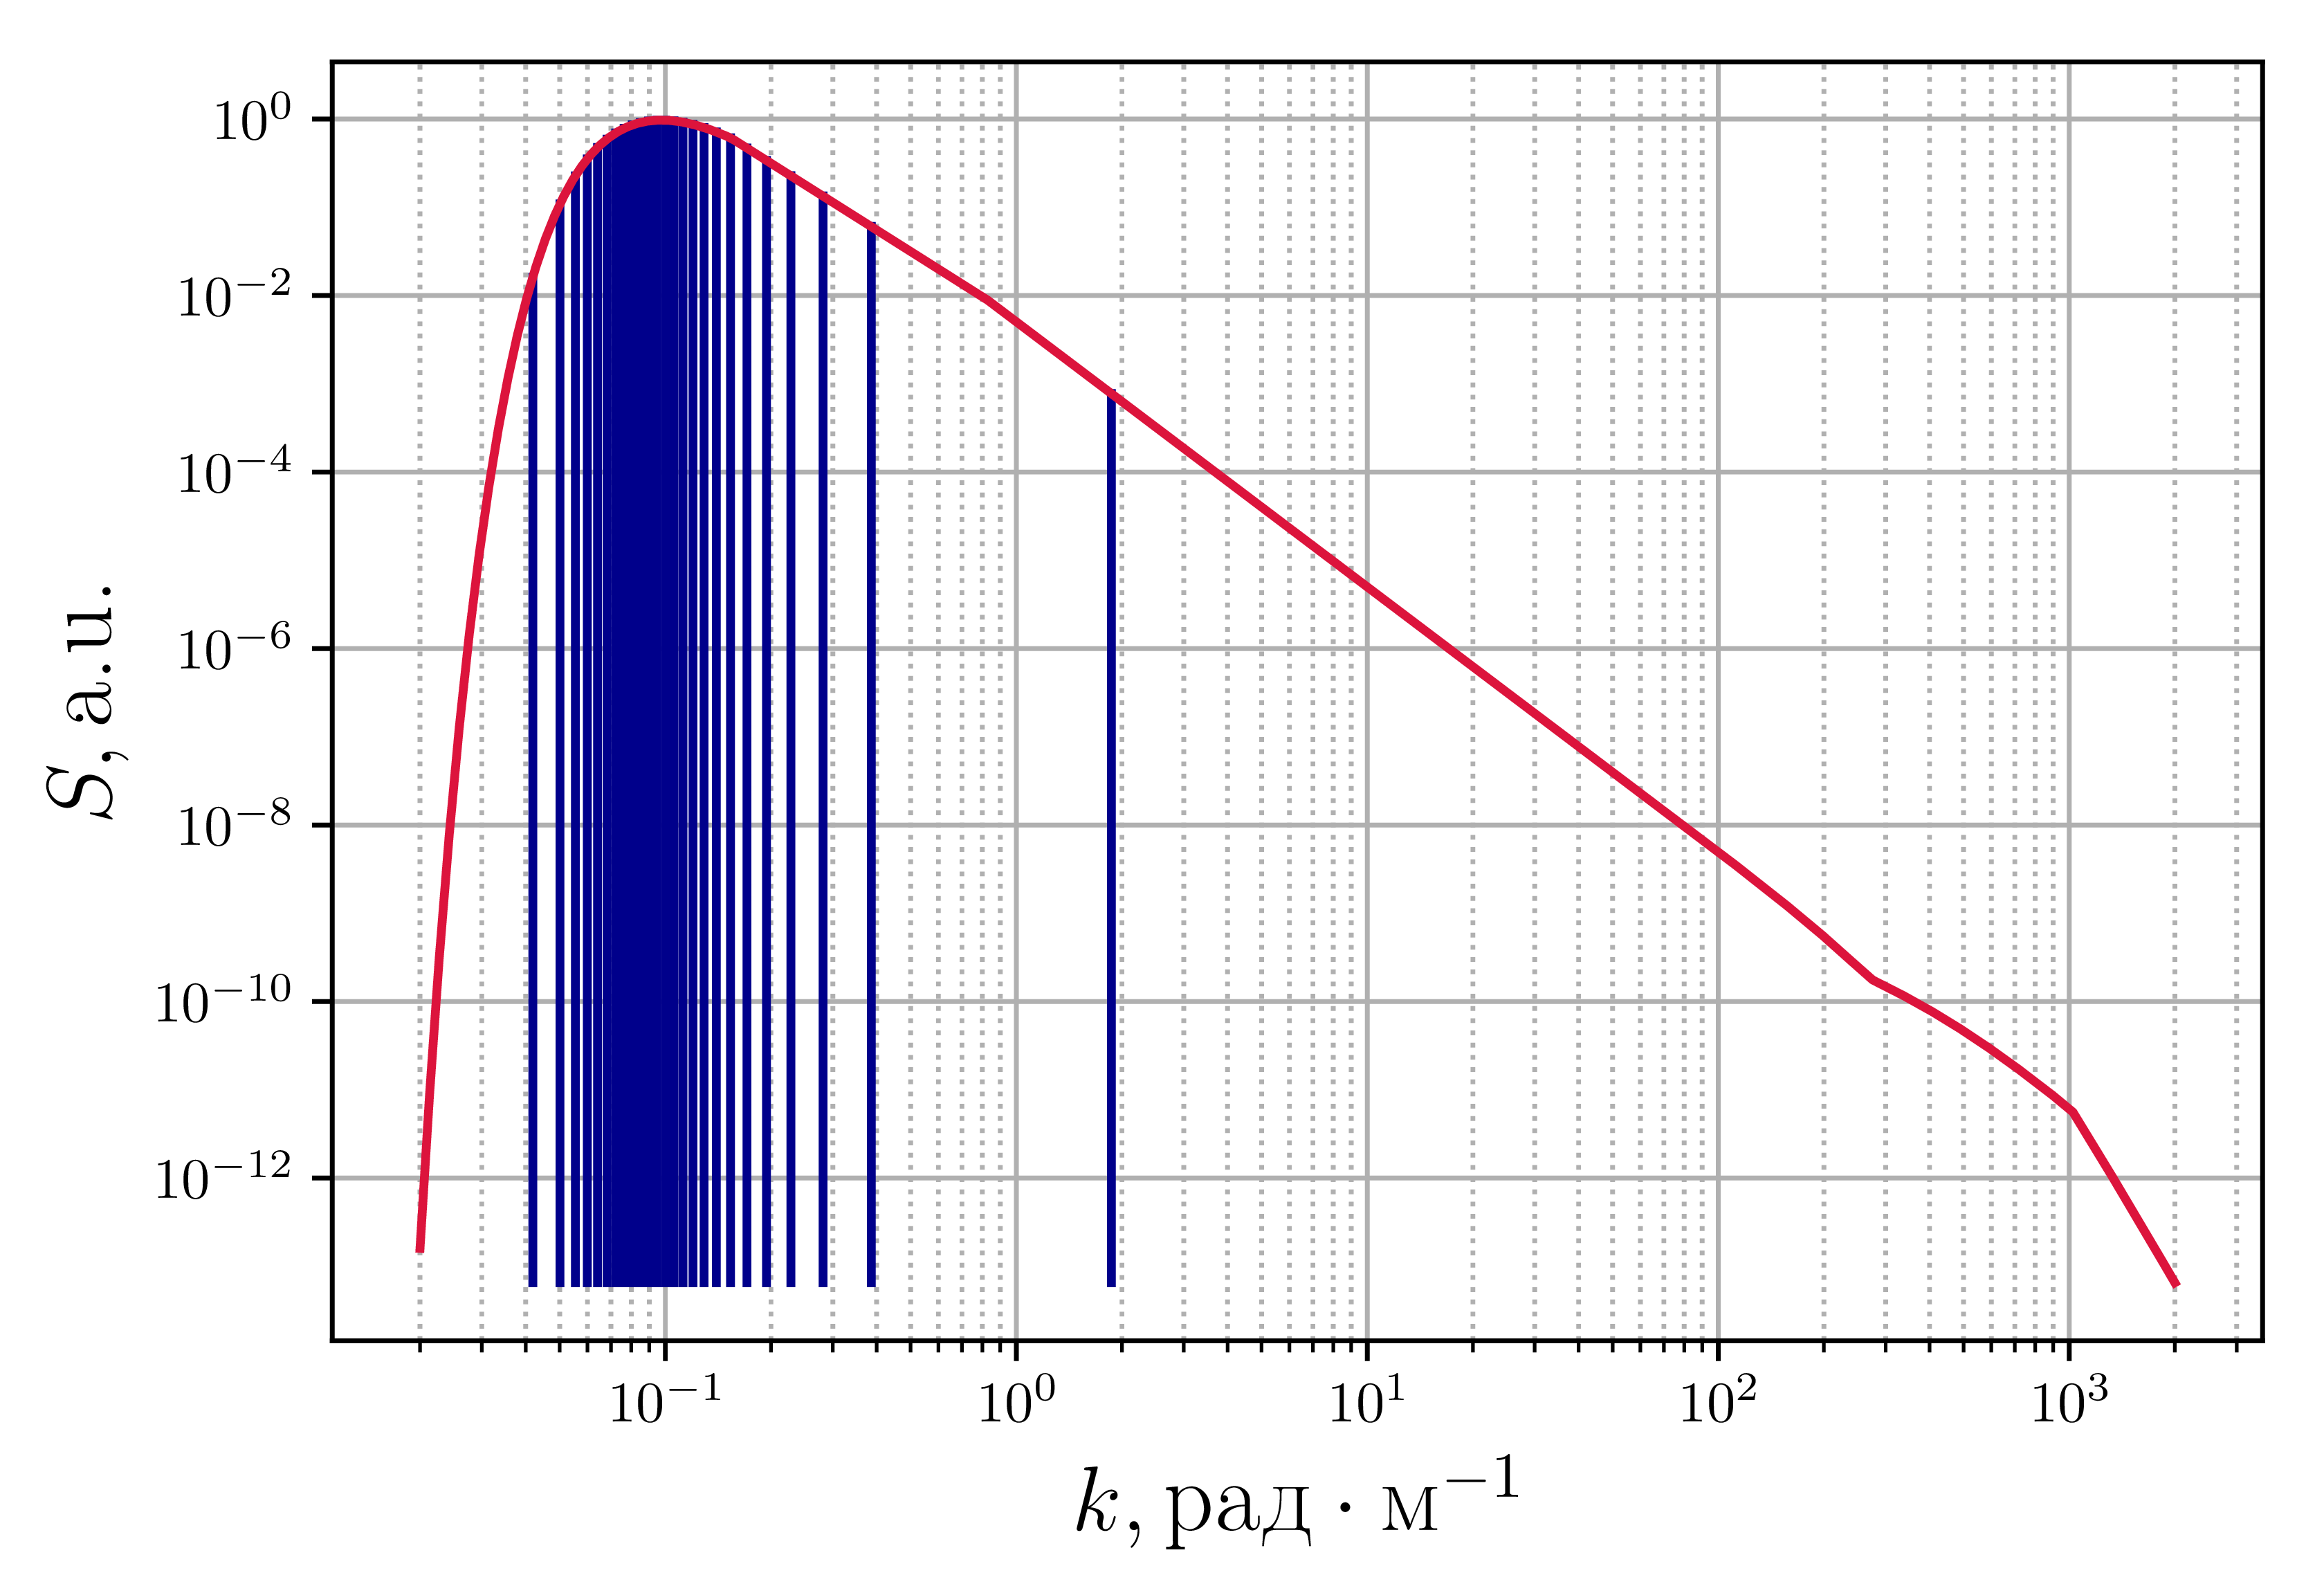
\includegraphics[width=\linewidth]{fig/split_height}
	\end{minipage}
	\caption{Расположении узлов по методу <<отбеливания>> спектра  для наклонов и высот соответственно. $U=10 \frac{\text{м}}{c}$, $N=25$}
	\label{fig:splits}		
\end{figure}

\end{frame}


\begin{frame}[plain]
	
	\frametitle{Сравнение методов}

   \begin{figure}[h!]
	\begin{minipage}{0.49\linewidth}
			\centering
			%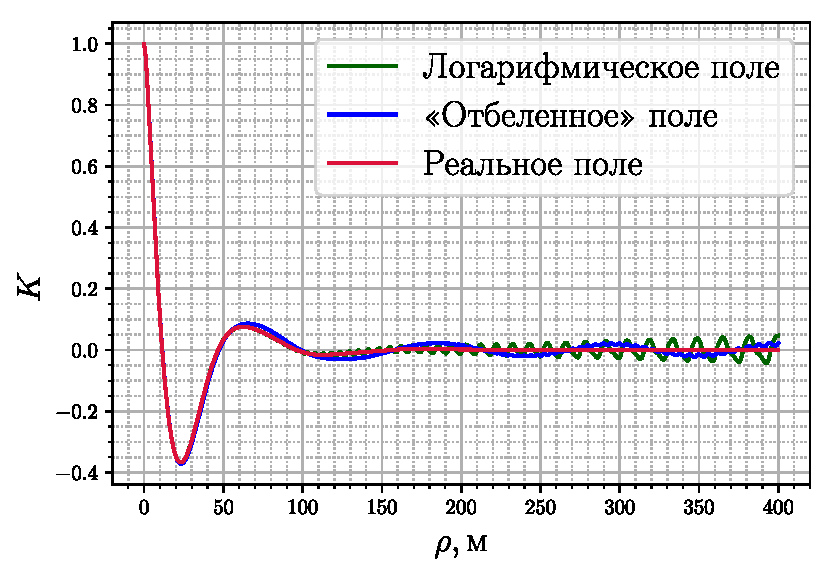
\includegraphics[width=\linewidth]{fig/correlation_height_wa.pdf}
			\label{fig:ch21}		
	\end{minipage}
	\hfill
	\begin{minipage}{0.49\linewidth}
			\centering
			%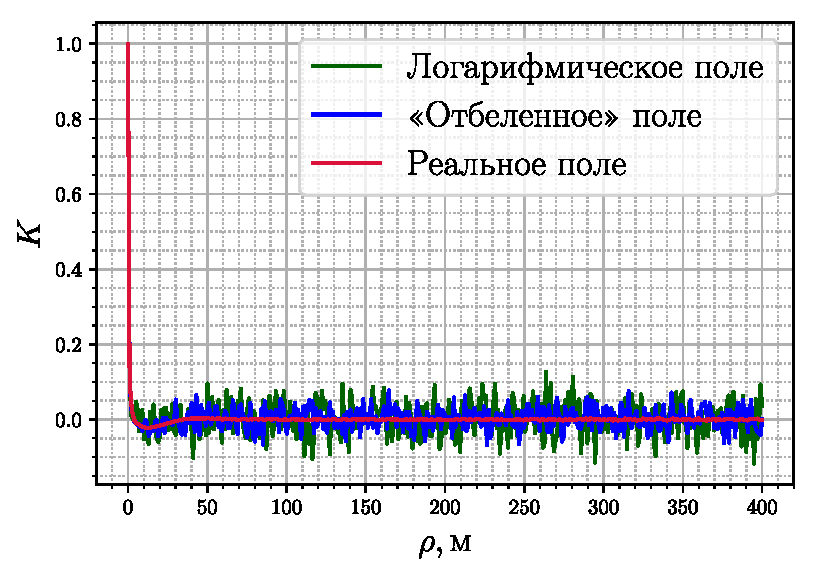
\includegraphics[width=\linewidth]{fig/correlation_angles_wa.pdf}
	\end{minipage}
	\caption{Корреляционные функции высот и уклонов при расположении узлов по методу <<отбеливания>> спектра для уклонов. $U=10 \frac{\text{м}}{\text{c}}$, $N=256$}
			\label{fig:ca21}		
\end{figure}

	Узлы задаются выражением
	\begin{equation}
	k_i=\sqrt\frac{N}{{\int\limits_{0}^{\infty} k^2 S(k) \dd{k}}}\cdot {\int\limits_{\Delta k_i} k^4 S(k) \dd{k}}
	\end{equation}



\end{frame}
\begin{frame}
	\frametitle{Двумерные функции корреляции}
	Для статистически однородного и стационарного поля справедливо следующее выражение для его корреляционной функции:
	\begin{equation}
		M(\vec \rho)= \iint\limits_{(\infty)} S(\vec k) \cos(\vec k \vec \rho) \dd{\vec k},
	\end{equation}
	где $S(\vec k)$-- волновой спектр морской поверхности.
	Корреляционную функцию наклонов морской поверхности определим как
	\begin{equation}
		M_{\theta} (\vec \rho) = \iint\limits_{(\infty)} k^2 \cdot S(\vec k) \cos(\vec k \vec \rho) \dd{ \vec k}
	\end{equation}
	Предположим, что переменные разделяются $S(\vec k)=S(k) \Phi_k(\phi)$,
	$k=\sqrt{k_x^2+k_y^2}$, $\phi=\arctg{\frac{k_y}{k_x}}$, а функция распределения нормирована на единицу $\int\limits_{-\pi}^{\pi} \Phi_k \dd{\phi}=1$
\end{frame}


\begin{frame}[t]

	\frametitle{Двумерная модель поверхностного волнения}
	Представим морскую поверхность в виде суммы синусоид с детерминированными амплитудами и случайными фазами:
\begin{equation}
	\zeta(\vec r, t)= \sum\limits_{n=1}^N \sum_{m=1}^M A_n(k_n)\cdot 
		\Phi_{k_nm}(\phi_m) \cos(\omega_n t + \vec k_n \vec r + \psi_{nm}),
\end{equation}
$\psi_{nm}$ -- случайная фаза, $A_n$ -- амплитуда $n$-ой гармоники.

Амплитуда, которая является мощностью на интервале $\Delta k_n$, вычисляется по спектру моделируемой поверхности
\begin{equation}
	A_n(k_n)=\sqrt{2 S(k_n) \Delta k_n}
\end{equation}

$\Phi_{nm}$ -- азимутальное распределение, вычисляемое следующим образом:
\begin{equation}
	\Phi_{nm}(k_n,\phi_m)=\sqrt{\Phi(k_n,\phi_m) \Delta \phi},
\end{equation}
$\Delta \phi$ -- шаг по углу.

\end{frame}
\begin{frame}[t]{Изображение поверхностей}
    \begin{figure}[h]
        \begin{subfigure}{0.49\linewidth}
            \centering
            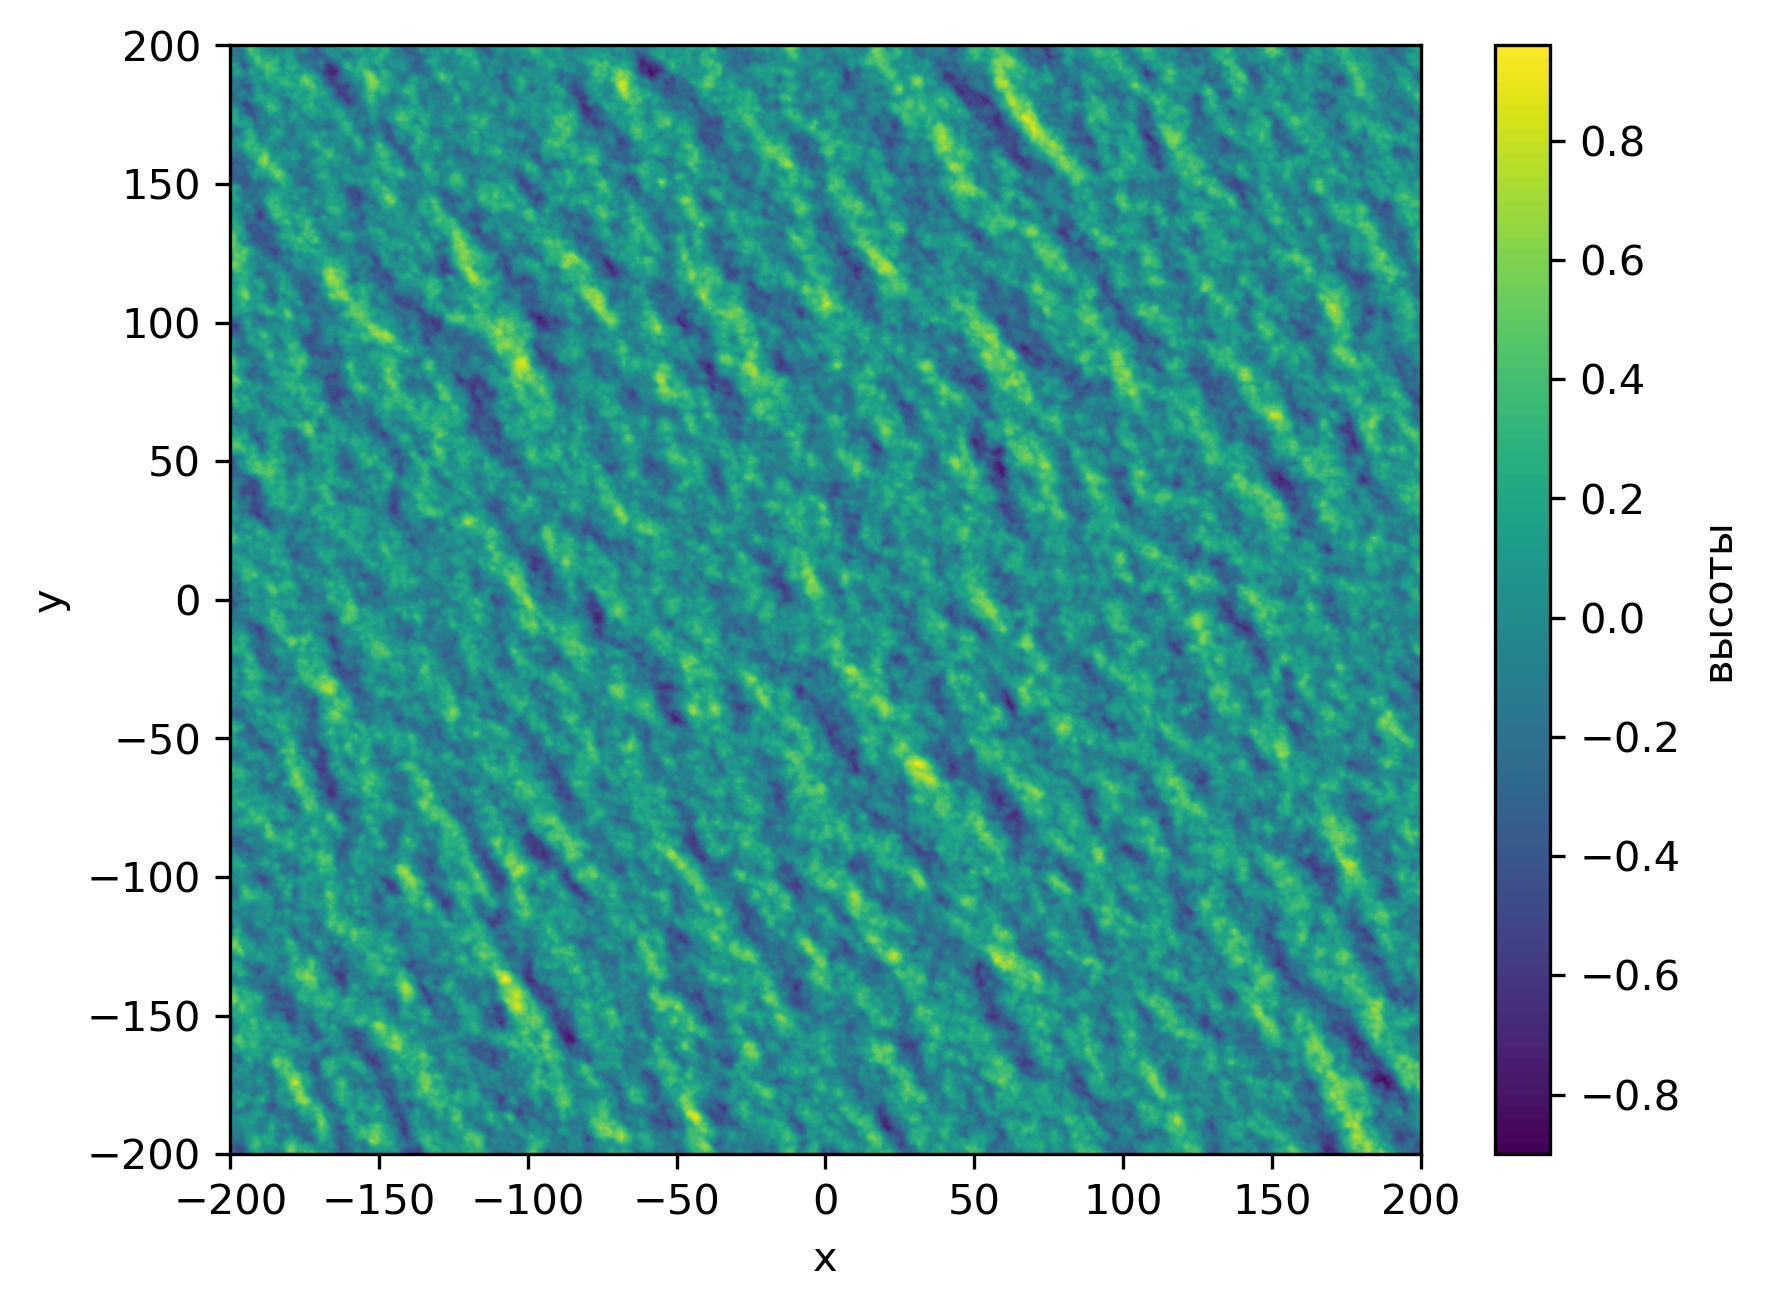
\includegraphics[width=1\linewidth]{img/heights5.png}
        \end{subfigure}
        \begin{subfigure}{0.49\linewidth}
            \centering
            \includegraphics[width=1\linewidth]{example-image-a}
        \end{subfigure}
        \begin{subfigure}{0.49\linewidth}
            \centering
            \includegraphics[width=1\linewidth]{example-image-a}
        \end{subfigure}
        \begin{subfigure}{0.49\linewidth}
            \centering
            \includegraphics[width=1\linewidth]{example-image-a}
        \end{subfigure}
    \end{figure}    
\end{frame}
\begin{frame}[t]
	\frametitle{Увеличение производительности}
    \begin{figure}[h]
        \begin{subfigure}{0.49\linewidth}
            \centering
            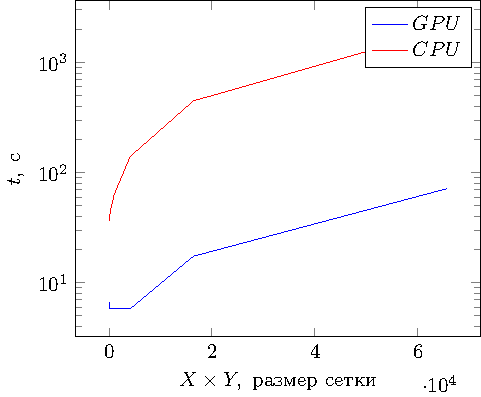
\includegraphics[width=\linewidth]{fig/water/gpucpu.pdf}
        \end{subfigure}
        \begin{subfigure}{0.49\linewidth}
            \centering
            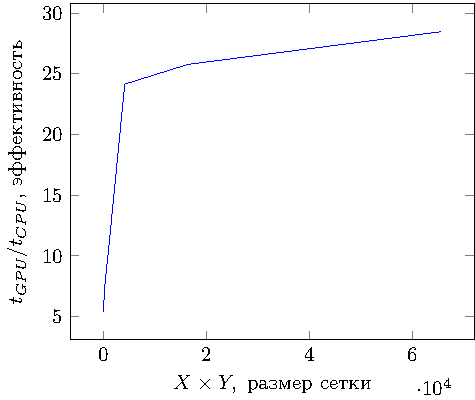
\includegraphics[width=\linewidth]{fig/water/gpucpu1.pdf}
        \end{subfigure}
    \end{figure}
\end{frame}


\begin{frame}[t]
	\frametitle{Моделирование отраженного импульса}
    \begin{figure}[h]
        \centering
        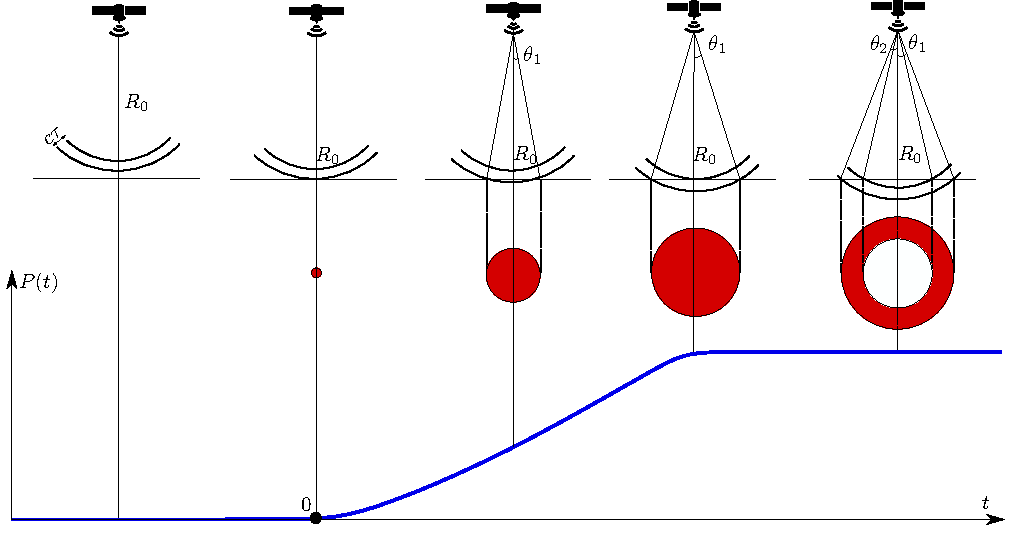
\includegraphics[width=\linewidth]{fig/flat_wave1.pdf}
    \end{figure}
\end{frame}

\begin{frame}[t]
	\frametitle{Моделирование отраженного импульса}
    \begin{figure}[h]
        \centering
        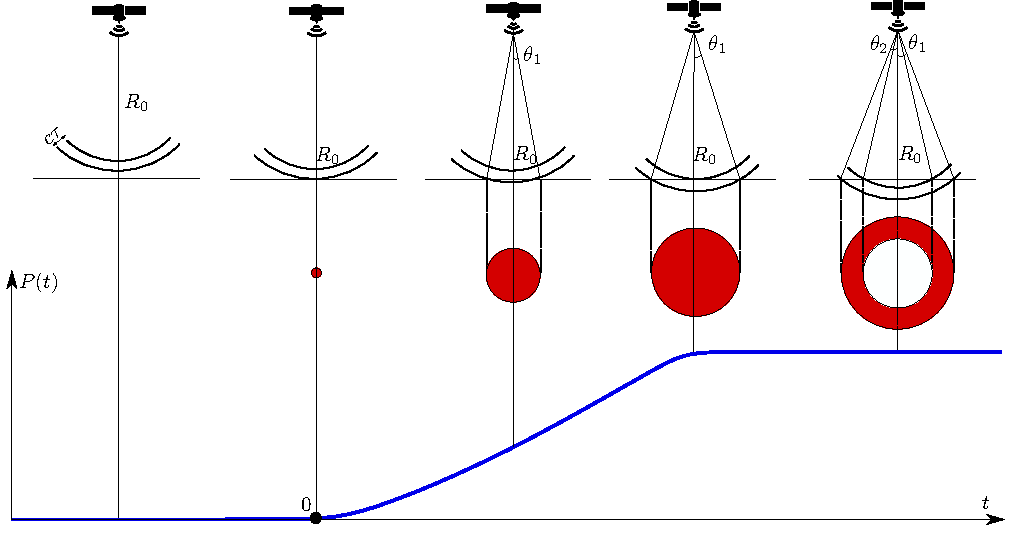
\includegraphics[width=\linewidth]{fig/flat_wave1.pdf}
    \end{figure}


	\begin{minipage}{0.49\linewidth}
        \begin{equation}
            brown formule
        \end{equation}
	\end{minipage}
	\hfill
	\begin{minipage}{0.49\linewidth}
        \begin{equation}
            ice formule
        \end{equation}
	\end{minipage}
\end{frame}

\begin{frame}[t]
	\frametitle{Моделирование отраженного импульса}
    \begin{figure}[h]
        \begin{subfigure}{\linewidth}
            \centering
            \def\svgwidth{0.8\linewidth}
            \includesvg{local_theta}
        \end{subfigure}
    \end{figure}
\end{frame}
\begin{frame}[t]
	\frametitle{Моделирование отраженного импульса}
    \begin{figure}[h]
        \begin{subfigure}{0.60\linewidth}
            \centering
            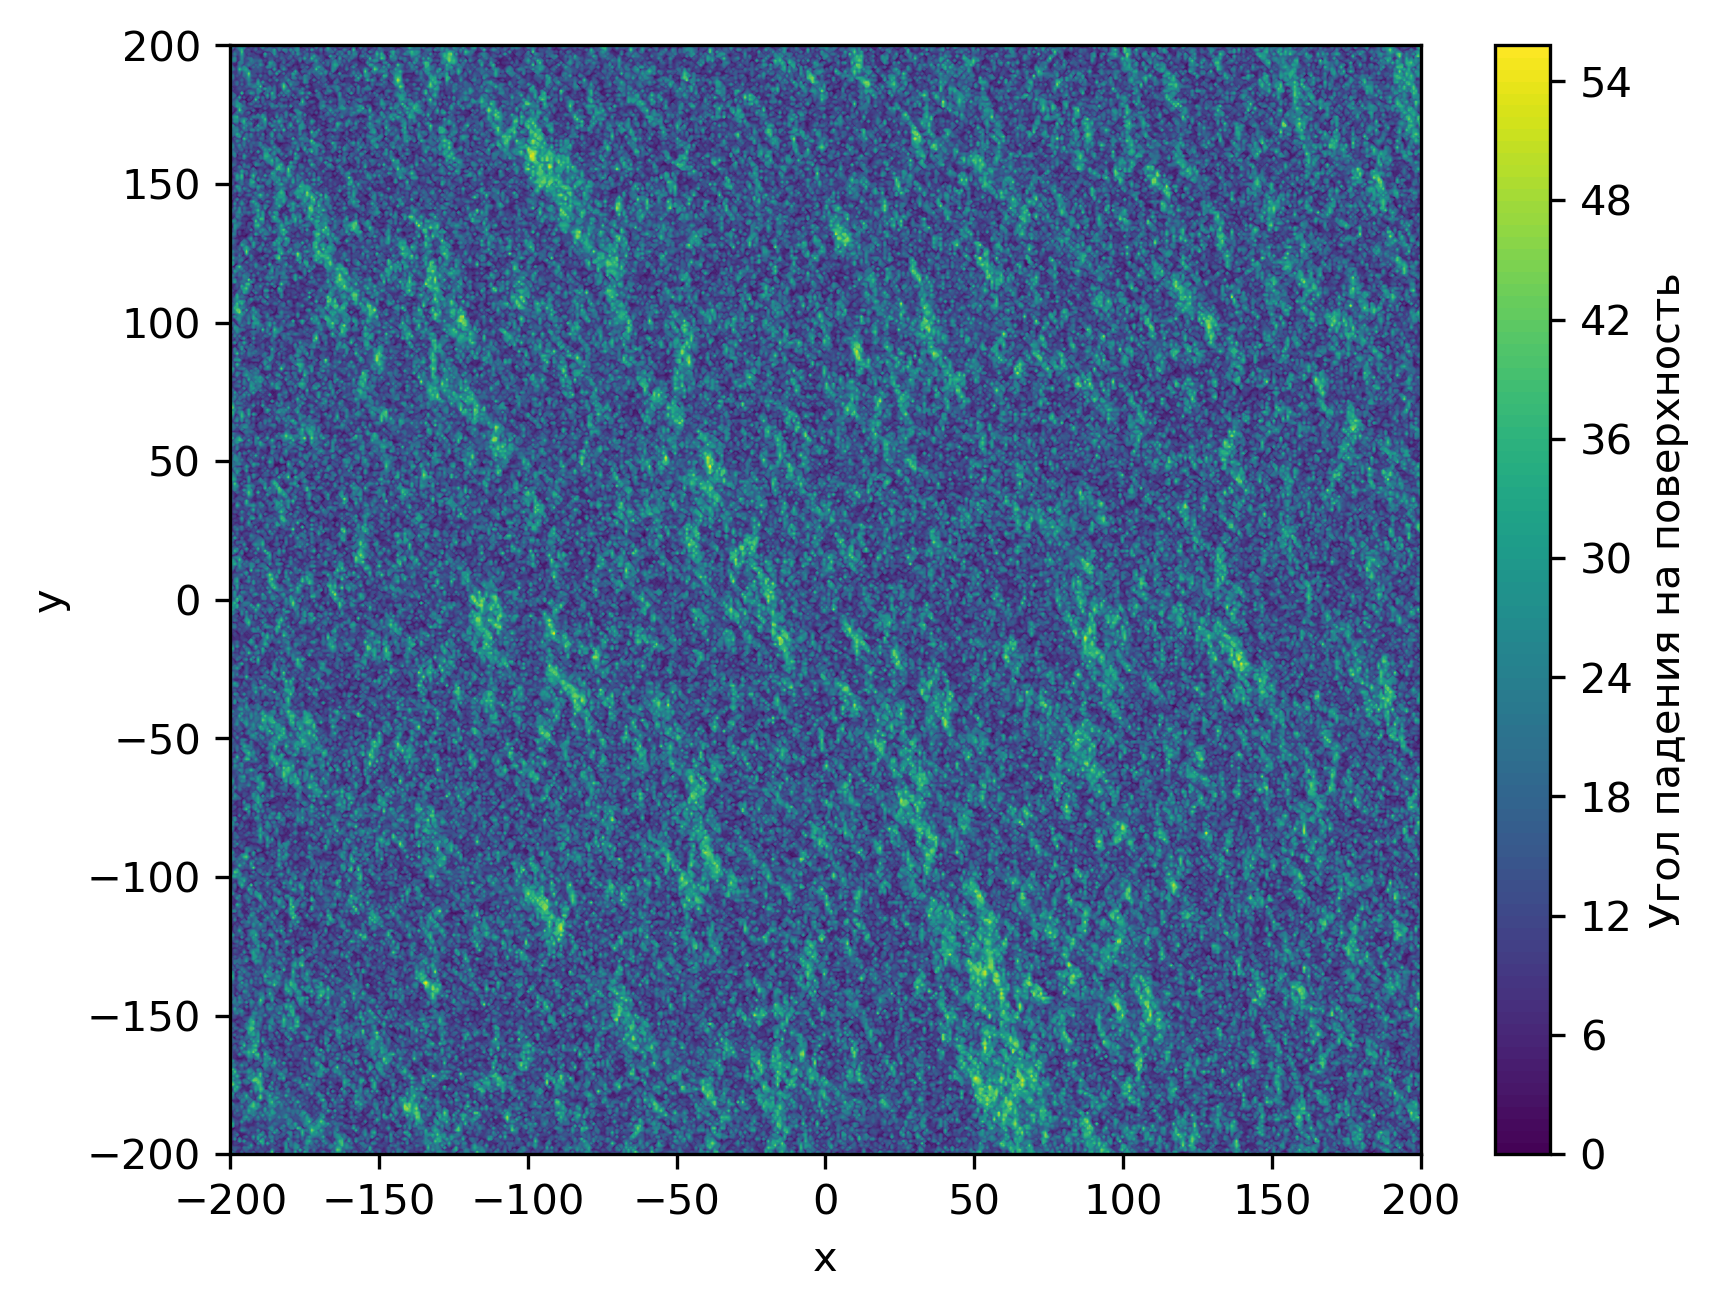
\includegraphics[width=\linewidth]{img/theta0}
        \end{subfigure}
        \begin{subfigure}{0.39\linewidth}
            \centering
            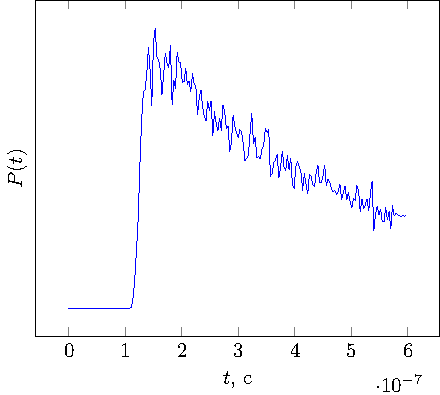
\includegraphics[width=\linewidth]{fig/theta}
        \end{subfigure}
    \end{figure}
\end{frame}
% \begin{frame}[t]\frametitle{Модель поверхностного волнения}
    
% \begin{figure}[h!]
% \begin{minipage}[h]{0.45\linewidth}
% 	\centering
% 	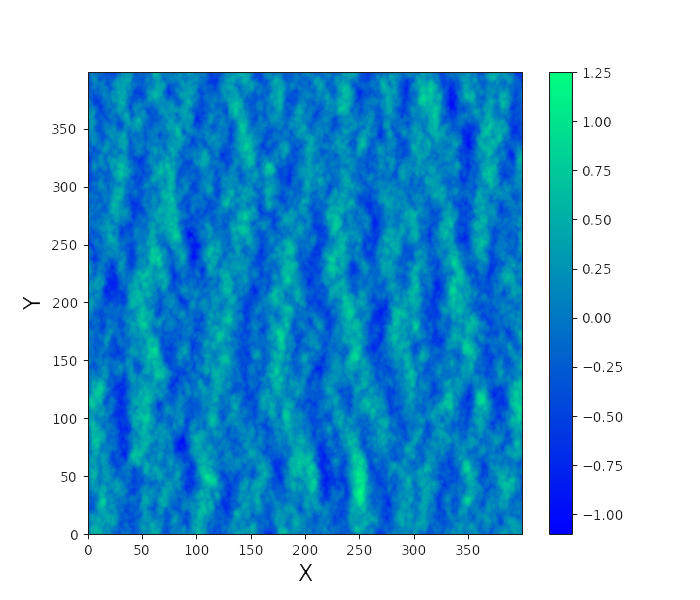
\includegraphics[width=\linewidth]{img/water7.png}
% 	% \caption{Моделирование высот морского волнения. $N=256, ~ U_{10}=7$  }
% 	\label{fig:water7}
% \end{minipage}
% \hfill
% \begin{minipage}[h]{0.45\linewidth}
% 	\centering
% 	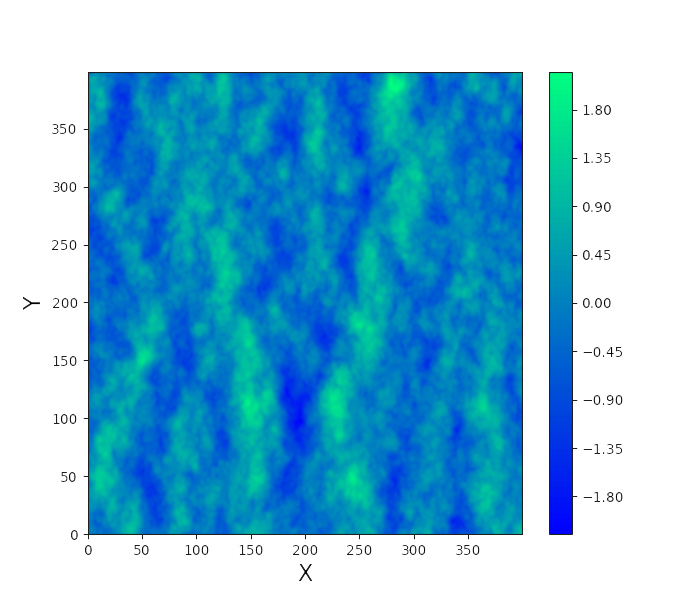
\includegraphics[width=\linewidth]{img/water10.png}
% 	% \caption{Моделирование высот морского волнения. $N=256, ~ U_{10}=10$ }
% 	\label{fig:water10}
% \end{minipage}
% \end{figure}

% \end{frame}
\begin{frame}
\frametitle{Форма импульса}
\vskip -3pt
    \begin{figure}[h]
        \centering
        \def\svgwidth{0.8\linewidth}
        \includesvg{example_impulse1}
        \caption{Качественная форма импульса с обозначением основных параметров.}
        \label{fig:impuls}
    \end{figure}
\end{frame}

\begin{frame}
\frametitle{Алгоритм ретрекинга}
\vskip -3pt
\def\imp{fig/retracking}
\begin{figure}
    \centering
    \begin{subfigure}{0.49\linewidth}
        \centering
        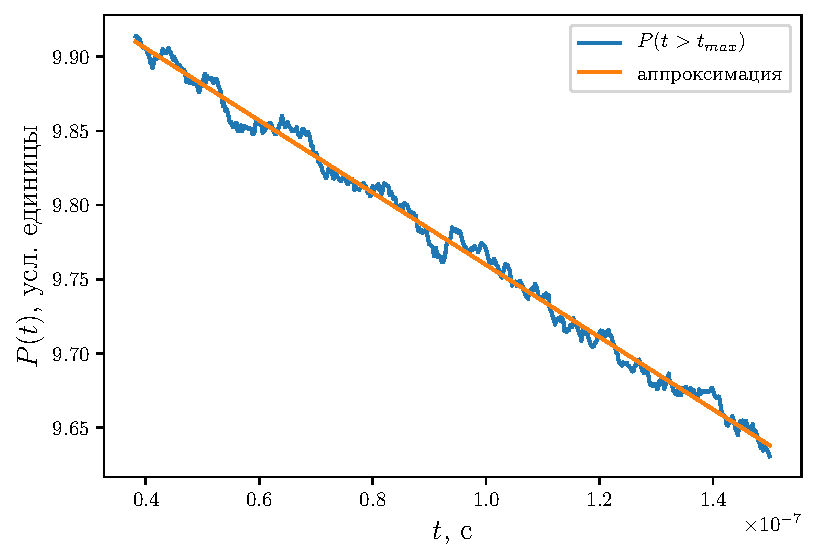
\includegraphics[width=1\linewidth]{\imp/imp_5_1}
    \end{subfigure}
    \begin{subfigure}{0.49\linewidth}
        \centering
        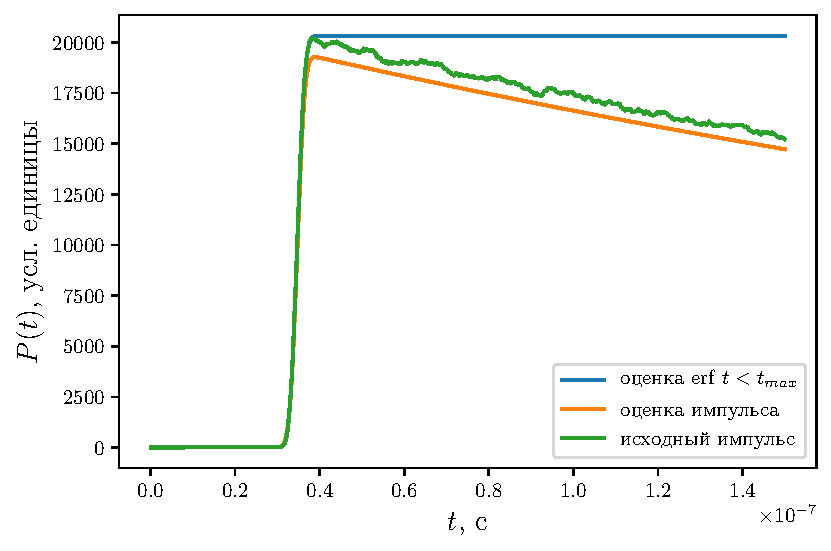
\includegraphics[width=1\linewidth]{\imp/imp_5_2}
    \end{subfigure}
    \begin{subfigure}{0.49\linewidth}
        \centering
        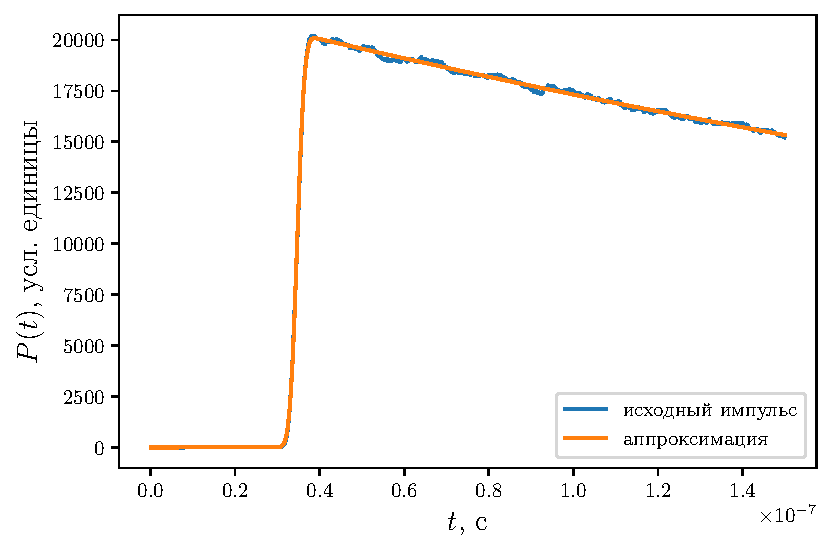
\includegraphics[width=1\linewidth]{\imp/imp_5_3}
    \end{subfigure}
\end{figure}
\end{frame}

\begin{frame}
\frametitle{Ретрекинг модельных импульсов}
\vskip -3pt
\begin{figure}
    \centering
    \begin{subfigure}{0.42\linewidth}
        \centering
        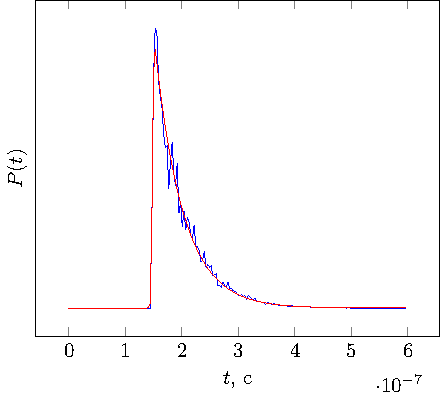
\includegraphics[width=1\linewidth,page=1]{fig/retracking/model}
    \end{subfigure}
    \begin{subfigure}{0.42\linewidth}
        \centering
        \includegraphics[width=1\linewidth,page=2]{fig/retracking/model}
    \end{subfigure}
    \begin{subfigure}{0.42\linewidth}
        \centering
        \includegraphics[width=1\linewidth,page=3]{fig/retracking/model}
    \end{subfigure}
\end{figure}
\end{frame}

\begin{frame}
\frametitle{Ретрекинг импульсов с Jason-3}
\vskip -3pt
\begin{figure}[ht]
    \centering
    \begin{subfigure}{0.42\linewidth}
        \centering
        \includegraphics[width=\linewidth, page=4]{fig/retracking5}
    \end{subfigure}
    \begin{subfigure}{0.42\linewidth}
        \centering
        \includegraphics[width=\linewidth, page=5]{fig/retracking5}
    \end{subfigure}
    \begin{subfigure}{0.42\linewidth}
        \centering
        \includegraphics[width=\linewidth, page=6]{fig/retracking5}
    \end{subfigure}
    %\caption{Форма отраженного импульса в зависимости от времени, полученного с
    %радиовысотомера космической миссии Jason-3.}
    \label{fig:impulse_jason}
\end{figure}
\end{frame}

\begin{frame}

\frametitle{Заключение}
\vskip -3pt
\begin{figure}
	%\animategraphics[autoplay,loop,width=0.8\linewidth]{15}{anim/water}{0}{360}
\end{figure}
\end{frame}

\end{document}
